\documentclass[xcolor=pdftex,dvipsnames,table,aspectratio=169]{beamer}
%\documentclass[xcolor=pdftex,dvipsnames,table,handout,aspectratio=169]{beamer}

%\setbeameroption{show notes}

\usepackage{bm,graphicx,multirow,amsmath,tikz} %fancybox,
\usepackage{color}%,textpos}
\usepackage[round]{natbib}
\usepackage[normalem]{ulem}
\usepackage{hyperref}
\usepackage{lastpage}
\usepackage{array}
\usepackage{color}
\usepackage{framed}
\usepackage{hyperref}

% Define Western colours
\definecolor{western}{rgb}{.306,.152,.524}
\definecolor{westerngray}{rgb}{.512,.508,.524}

%% Define BEAMER colours
\setbeamercolor{frametitle}{bg=western,fg=white}
\setbeamercolor{framesubtitle}{bg=western,fg=black}
\setbeamercolor{title}{fg=white,bg=western}
\setbeamercolor{author}{fg=white,bg=western}
\setbeamercolor{institute}{fg=white,bg=western}
\setbeamercolor{date}{fg=white,bg=western}

%% Set BEAMER fonts
\setbeamerfont{title}{shape=\bf}
\setbeamerfont{frametitle}{shape=\sc,size=\Large}
\setbeamerfont{framesubtitle}{shape=\sc,size=\Large}
\setbeamerfont{footline}{shape=\sc}

%% Define BEAMER toc
\setbeamercolor{section in toc}{fg=western}
\setbeamercolor{subsection in toc}{fg=westerngray}
\setbeamertemplate{sections/subsections in toc}[ball]

%% Define BEAMER background
\setbeamercolor{background canvas}{bg=white}

%% Define BEAMER footer
\setbeamertemplate{navigation symbols}{}
\setbeamercolor{footline}{fg=white,bg=western}
\setbeamertemplate{footline}{%
  \begin{beamercolorbox}[wd=\paperwidth]{footline}
    \vskip5pt

    \raisebox{.05in}{
      \scriptsize{\bf \insertshorttitle}
    }
    \hfill
    \raisebox{.05in}{
      \scriptsize{\bf \insertframenumber/\inserttotalframenumber} 
    }
    \hspace{5pt}

    \vskip5pt
  \end{beamercolorbox}
}

%% Define BLOCK environment
\setbeamercolor{block title}{fg=western}
\setbeamerfont{block title}{series=\bfseries}

%% Define ENUMERATE and ITEMIZE environements
\setbeamertemplate{itemize item}[ball]
\setbeamertemplate{enumerate item}[ball]
\setbeamercolor{item projected}{bg=western}

%% Define BEAMER toc
\setbeamercolor{sections/subsections in toc}{fg=blue!75}
\setbeamertemplate{sections/subsections in toc}[ball]

% %% Define SECTION openings
% \AtBeginSection[]{
%   \begin{frame}{\insertshorttitle}
%     \tableofcontents[currentsection,subsectionstyle=hide/hide/hide]
    
%   \end{frame}
% }

%% Define BEAMER frametitle
\addtobeamertemplate{frametitle}{
   \let\insertframetitle\insertsectionhead}{}
\addtobeamertemplate{frametitle}{
   \let\insertframesubtitle\insertsubsectionhead}{}


\makeatletter
  \CheckCommand*\beamer@checkframetitle{\@ifnextchar\bgroup\beamer@inlineframetitle{}}
  \renewcommand*\beamer@checkframetitle{\global\let\beamer@frametitle\relax\@ifnextchar\bgroup\beamer@inlineframetitle{}}
\makeatother

% Define counters for example and exercise
\newcounter{example}
\newcounter{exercise}

% Define example and exercise commands
\renewcommand{\example}
{\stepcounter{example}Example \lecturenum.\arabic{example}}
\newcommand{\examplectd}
{Example \lecturenum.\arabic{example}\ ctd}
\newcommand{\exercise}
{\stepcounter{exercise}Exercise \lecturenum.\arabic{exercise}}
\newcommand{\exercisectd}
{Exercise \lecturenum.\arabic{exercise}\ ctd}

\newcommand{\lecturenum}{20}

\title[SS2857]{Probability and Statistics I}
\subtitle{\lecturenum.~Jointly Distributed Random Variables}

\date{}

%% Add logo
%% \titlegraphic{\includegraphics[height=2cm]{../uwo_logo_reversed}}

%% Initialize R


\begin{document}

{
\setbeamertemplate{footline}{}
\setbeamercolor{background canvas}{bg=western}

\begin{frame}
  \addtocounter{framenumber}{-1}

  \maketitle
\end{frame}
}

\section{Review Exercise}

\begin{frame}
  \frametitle{\invisible{Hello}}
  
  \begin{center}
    \Large{\textbf{5.1 Jointly Distributed Random Variables}}

    \bigskip

    \Large{Discrete Random Variables}
  \end{center}
  
\end{frame}

\section{Review: Conditional Probabilities}

\begin{frame}

Recall that the conditional probability of the event $A$ given $B$ is:
$$
P(A|B)=\frac{P(A \cap B)}{P(B)}.
$$

\bigskip

The two events are independent if
$$
P(A|B)=P(A), \quad P(B|A)=P(A), \mbox{ or } P(A \cap B)=P(A)P(B).
$$
\end{frame}

\section{Discrete Random Variables}

\label{sec:two-discrete-random}

\begin{frame}
  \begin{block}{Joint Probability Mass Function}
    Let $X$ and $Y$ be two discrete random variables defined on the sample space $\mathcal S$. The joint probability mass function $p(x,y)$ is defined for each pair of numbers $(x,y)$ by
    \[
      p(x,y)=P(X=x\mbox{ and } Y=y)=P(X=x,Y=y).
    \]
  \end{block}
\end{frame}

\begin{frame}
  \begin{block}{Examples}
  
  Let $\mathcal S$ be the set of days in 2024.
  
  $$
  X=
  \left\{
  \begin{array}{ll}
  0 & \mbox{it doesn't snow}\\
  1 & \mbox{it snows}\\
  \end{array}
  \right.
  $$
  and
  $$
  Y =\mbox{Month of year (1=Jan, 2=Feb,$\ldots$,12=Dec)}
  $$
  \end{block}
\end{frame}

\begin{frame}
  \begin{block}{Examples}
  
  Let $\mathcal S$ be the set of days in cards in a standard deck.
  
  $$
  X=\mbox{value (1=A,2=2,3=3,$\ldots$,11=J,12=Q,13=K)}
  $$
  and
  $$
  Y =\mbox{suit (1=Clubs, 2=Diamonds, 3=Hearts, 4=Spades)}
  $$
  \end{block}
\end{frame}

\begin{frame}
  \begin{block}{Examples}
  
  Let $\mathcal S$ be all possible outcomes of rolling two die (e.g., (1,1) or (3,2)).
  
  $$
  X=\mbox{sum of the two values}
  $$
  and
  $$
  Y =\mbox{difference of the two values}
  $$
  \end{block}
\end{frame}

\begin{frame}
  \begin{block}{Marginal Probability Mass Function}
    The marginal probability mass functions of $X$ and $Y$, denoted $p_X(x)$ and $p_Y(y)$, are given by
    \[
      p_X(x)=\sum_{y}p(x,y) \mbox{ and } p_Y(y)=\sum_xp(x,y).
    \]

    \bigskip

    Note that this should really say:
    \[
      p_X(x)=\sum_{y \in \mathcal{Y}}p(x,y) \mbox{ and } p_Y(y)=\sum_{x \in \mathcal{X}} p(x,y)
    \]
    where $\mathcal{X}$ and $\mathcal{Y}$ represent the range of $X$ and $Y$, respectively.
    
  \end{block}
\end{frame}

\begin{frame}
  \begin{block}{Independence}
    Two discrete random variables $X$ and $Y$ are said to be independent if
    \[
      p(x,y)=p(x)p(y)
    \]
    for every $x \in \mathcal{X}$ and $y \in \mathcal{Y}$. 
    
    \bigskip
    
    If $X$ and $Y$ are not independent, then they are dependent. 
  \end{block}
\end{frame}



\begin{frame}
  \begin{block}{\example: Berkeley Admissions Data}
    The following data come from a study conducted at UC Berkeley in the 1970's to assess claims of bias in graduate admissions. The data contain records from 4256 applicants to the top six different degrees (Majors). The names of the degrees were kept confidential.
    
    \begin{center}
      \begin{tabular}{lcc}
        & \multicolumn{2}{c}{Applicants by Gender}\\
        Major & Men & Women\\
        \hline
        A & 825 & 108\\
        B & 560 & 25\\
        C & 325 & 593\\
        D & 417 & 375\\
        E & 191 & 393\\
      F & 373 & 341\\
      \end{tabular}
    \end{center}
  \end{block}
\end{frame}

\begin{frame}
  \begin{block}{\examplectd}
    Define the random variables
    \[
    X=
    \left\{
      \begin{array}{ll}
        0 & \mbox{an applicant is male}\\
        1 & \mbox{an applicant is female}
      \end{array}
    \right.
    \]
    \[
    Y=
    \left\{
      \begin{array}{ll}
        1 & \mbox{an applicant applies to Major A}\\
        \vdots &\\
        6 & \mbox{an applicant applies to Major F}
      \end{array}
    \right.
    \]
    
    \begin{enumerate}[a)]
    \item Estimate the joint pmf of $X$ and $Y$. 
    \item Compute the marginal distributions of $X$ and $Y$. 
    \item Are $X$ and $Y$ independent? What would this mean?
    \end{enumerate}
  \end{block}
\end{frame}

\begin{frame}
  \begin{block}{\examplectd}
% latex table generated in R 4.4.1 by xtable 1.8-4 package
% Wed Nov  6 11:28:53 2024
\begin{table}[ht]
\centering
\begin{tabular}{rlrr}
  \hline
 & Major & Men & Women \\ 
  \hline
1 & A & 0.182 & 0.024 \\ 
  2 & B & 0.124 & 0.006 \\ 
  3 & C & 0.072 & 0.131 \\ 
  4 & D & 0.092 & 0.083 \\ 
  5 & E & 0.042 & 0.087 \\ 
  6 & F & 0.082 & 0.075 \\ 
   \hline
\end{tabular}
\end{table}

\end{block}
\end{frame}

\begin{frame}
  \begin{block}{\examplectd}
    \begin{center}
      \begin{tabular}{lrr|r}
        \hline
        Major & Men & Women & $p_Y(y)$\\ 
        \hline
        A & 0.182 & 0.024 & .21\\ 
        B & 0.124 & 0.006 & .13\\ 
        C & 0.072 & 0.131 & .20\\ 
        D & 0.092 & 0.083 & .17\\ 
        E & 0.042 & 0.087 & .13\\ 
        F & 0.082 & 0.075 & .16\\ 
        \hline
        $p_X(x)$ & .59 & .41
      \end{tabular}
    \end{center}
  \end{block}
\end{frame}

\begin{frame}
  \begin{block}{\examplectd: $p(x,y)$}
    \begin{center}
      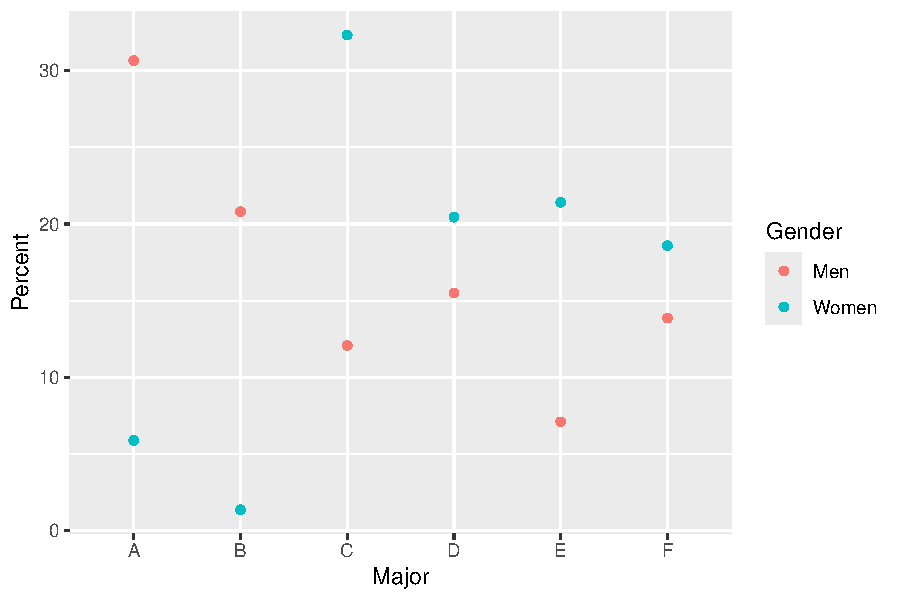
\includegraphics[height=.7\textheight]{figure/berkeley-1}
    \end{center}
  \end{block}
\end{frame}



\begin{frame}
  \begin{block}{\examplectd: $p(x)p(y)$}
    \begin{center}
      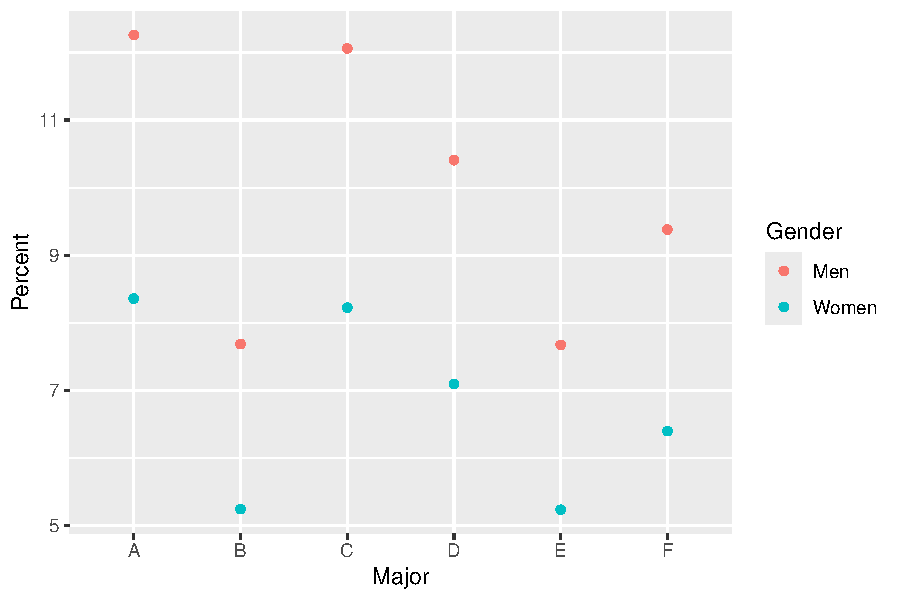
\includegraphics[height = .7\textheight]{figure/berkeley3-1}
    \end{center}
  \end{block}
\end{frame}

\section{Continuous Random Variables}

\begin{frame}
  \frametitle{\invisible{Hello}}
  
  \begin{center}
    \Large{\textbf{5.1 Jointly Distributed Random Variables}}

    \bigskip

    \Large{Continuous Random Variables}
  \end{center}
  
\end{frame}

\begin{frame}
  \begin{block}{Joint Probability Density Function}
    Let $X$ and $Y$ be two continuous random variables. Then $f(x,y)$ is the joint probability density function for $X$ and $Y$ if
    \[
      P[(X,Y) \in A]=\int \int_A f(x,y)~dx~dy
    \]
    for any set $A \in \mathbb R^2$. In particular, if $A$ is a rectangle with limits $a \leq x \leq b$ and $c \leq y \leq d$ then 
    \[
    P[(X,Y) \in A]=P(a \leq x \leq b, c \leq y \leq d)= \int_a^b \int_c^d f(x,y)~dx~dy.
    \]
  \end{block}
\end{frame}

\begin{frame}
  \begin{block}{Joint Probability Density Function}
  The function $f(x,y)$ is a valid joint pdf if 
  $$
  f(x,y)\geq 0 \mbox{ for all } (x,y) \in \mathbb R^2
  $$
  and 
  $$ 
  \int_{-\infty}^\infty \int_{-\infty}^{\infty} f(x,y)~dx~dy=1.
  $$
  \end{block}
\end{frame}


\begin{frame}
  \begin{block}{Marginal Probability Density Function}
    The marginal probability density functions of $X$ and $Y$, denoted $f_X(x)$ and $f_Y(y)$, are given by
    $$
      f_X(x)=\int_{-\infty}^{\infty}f(x,y)~dy
    $$
    and
    $$
    f_Y(y)=\int_{-\infty}^{\infty}f(x,y)~dx
    $$
    for $x,y \in (-\infty,\infty)$. 
    
  \end{block}
\end{frame}

\begin{frame}
  \begin{block}{Independence}
    Two continuous random variables $X$ and $Y$ are said to be independent if
    \[
      f(x,y)=f(x)f(y)
    \]
    for every $(x,y)\in \mathbb R^2$. 
    
    \bigskip
    
    If $X$ and $Y$ are not independent then they are dependent. 
  \end{block}
\end{frame}

\begin{frame}
  \begin{block}{\example}
    Suppose that $X$ and $Y$ have the joint pdf
    \[
      f(x,y)=
      \left\{
        \begin{array}{ll}
          c(1-x^2)(1-y^2) & -1 < x < 1\mbox{ and } -1 < y < 1\\
          0 & \mbox{otherwise}
        \end{array}
      \right.
    \]
    \begin{enumerate}[a)]
    \item Find the value of $c$ so that $f(x,y)$ is a proper pdf.
    \item Find the marginal distribution of $X$ and $Y$.
    \item Are $X$ and $Y$ independent? 
    \end{enumerate}
  \end{block}
\end{frame}






\begin{frame}
  \begin{block}{\examplectd}
    \begin{center}
      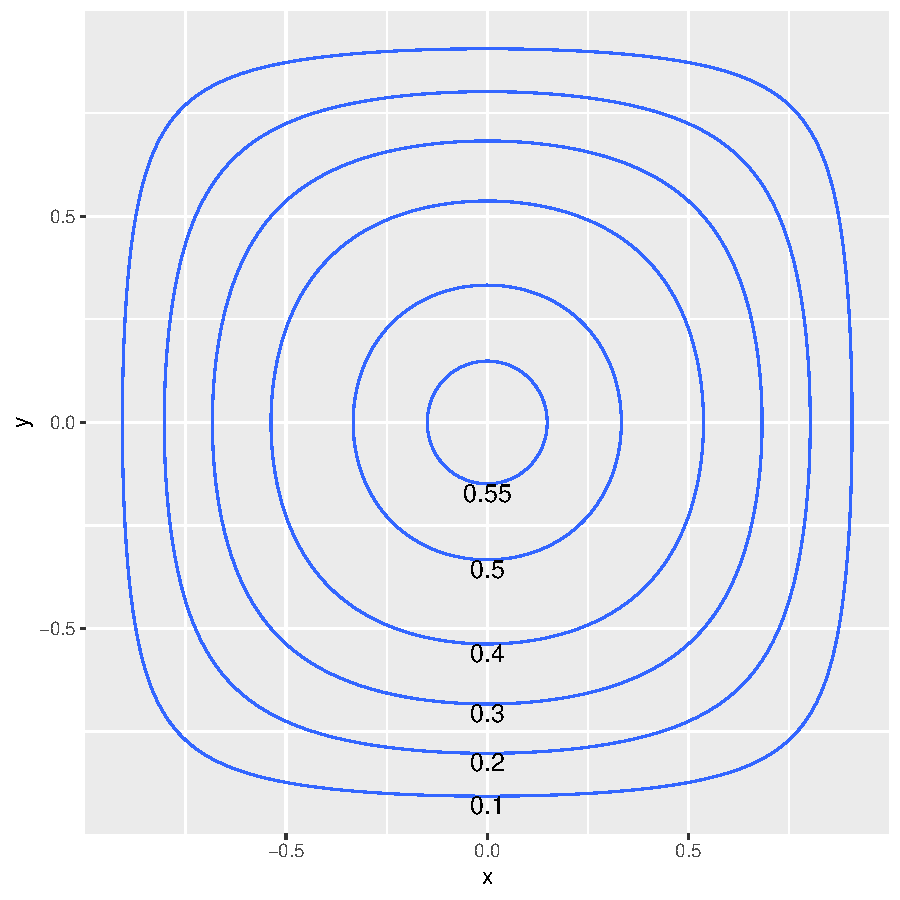
\includegraphics[height = .7\textheight]{figure/example2-1}
    \end{center}
  \end{block}
\end{frame}

\begin{frame}
  \begin{block}{\examplectd}
    \begin{center}
      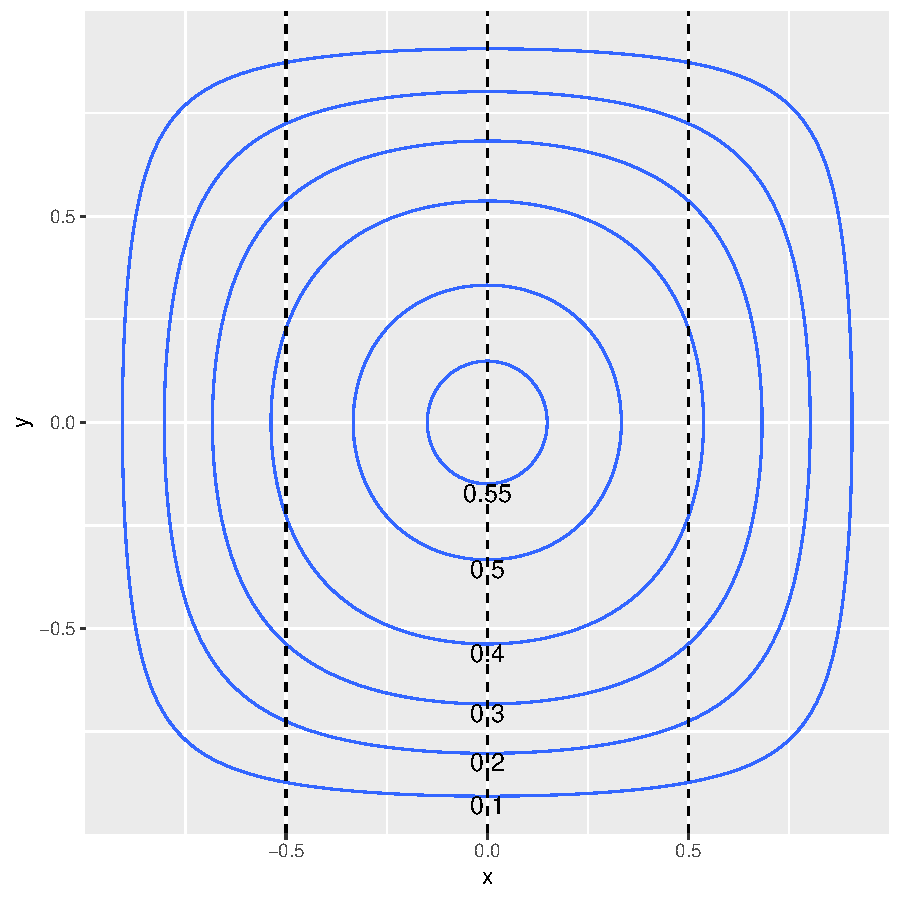
\includegraphics[height = .7\textheight]{figure/example2-2}
    \end{center}
  \end{block}
\end{frame}

\begin{frame}
  \begin{block}{\examplectd}
    \begin{center}
      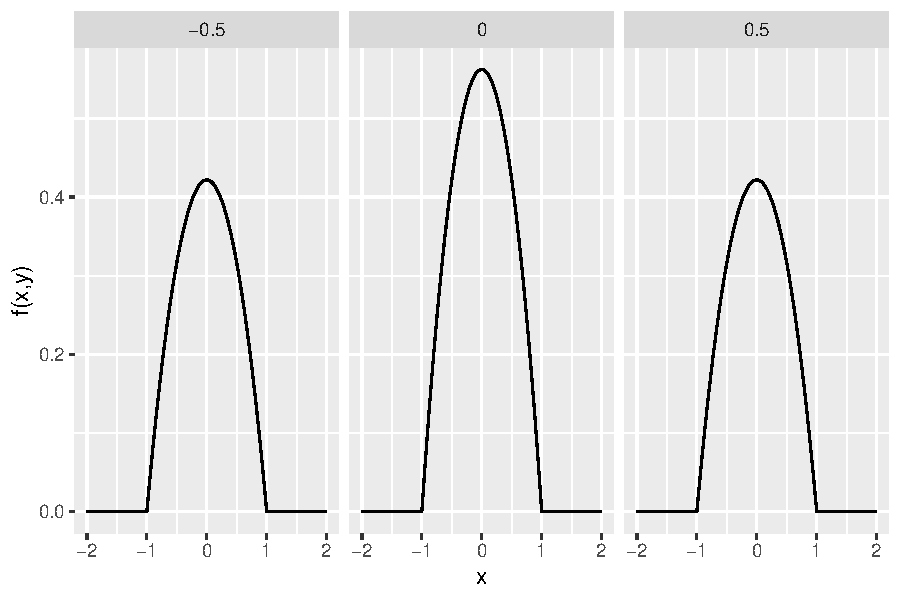
\includegraphics[height = .7\textheight]{figure/example2-1-1}
    \end{center}
  \end{block}
\end{frame}

\begin{frame}
  \begin{block}{\examplectd}
    \begin{center}
      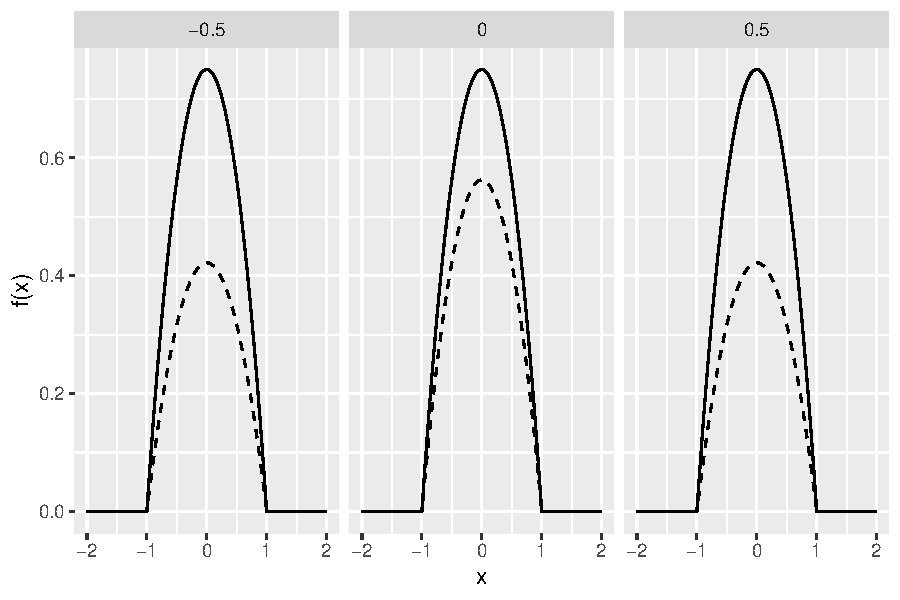
\includegraphics[height = .7\textheight]{figure/example2-1-2}
    \end{center}
  \end{block}
\end{frame}

\begin{frame}<handout:0>
  \begin{center}
    \Huge{\textbf{Questions?}}
  \end{center}
\end{frame}

\begin{frame}
  \begin{block}{\exercise}
  \begin{center}
  Suppose that
  $$
  f(x,y)=c \min(x,y), 0<x,y<1. 
  $$
  \begin{enumerate}[a)]
  \item Find the value $c$ so that $f(x,y)$ is a valid joint pdf.
  \item Compute $P(X > .5, Y > .5)$.
  \item Derive the marginal density of $X$ and $Y$.
  \item Are $X$ and $Y$ independent?
  \end{enumerate}
  \end{center}
  \end{block}
\end{frame}
\end{document}
